% Capítulo 4: Propuesta de solución
\section{Introducción}
\label{sec:prop-intro}

En el capítulo anterior se revisó el estado del arte de los sistemas multiagente basados en LLM para el diseño de circuitos analógicos, y se identificó que los trabajos reportados operan a nivel de transistor sobre un nodo tecnológico (PDK), mientras que la generación y validación de circuitos a nivel de componentes comerciales (COTS) con simulación SPICE dentro del lazo de diseño permanece como una brecha abierta. Este capítulo presenta la propuesta de solución que atiende esa brecha.

El propósito del capítulo es exponer el diseño del sistema antes de su construcción: las premisas que lo fundamentan, su descomposición funcional, su arquitectura estructural y su comportamiento en ejecución. Las decisiones de diseño se justifican a partir de la naturaleza del problema, de los principios de la ingeniería de software y de los hallazgos del estado del arte; los artefactos de análisis y diseño elaborados a lo largo del proyecto —la Especificación de Requisitos de Software (SRS), el modelo de casos de uso, el diagrama funcional, el modelo arquitectónico C4 de tres niveles y el diagrama de secuencia— registran y representan esas decisiones, de modo que cada una quede expresada en un artefacto verificable.

La exposición sigue un orden de lo abstracto a lo concreto. Primero se establecen el problema que el diseño debe resolver, las premisas que lo orientan y el papel del SRS como registro de los requisitos (sección~\ref{sec:prop-premisas}). A continuación se describe \textit{qué} hace el sistema mediante su descomposición funcional y sus casos de uso (sección~\ref{sec:prop-funcional}). Después se describe \textit{cómo} se estructura, mediante el modelo C4 en sus tres niveles (sección~\ref{sec:prop-c4}). Enseguida se describe \textit{cómo se comporta} en ejecución, mediante el diagrama de secuencia del flujo principal de generación (sección~\ref{sec:prop-dinamico}). Finalmente se explican los atributos de calidad y seguridad que se desprenden del diseño (secciones~\ref{sec:prop-calidad} y~\ref{sec:prop-seguridad}), se enuncian los criterios de aceptación que la propuesta deberá satisfacer (sección~\ref{sec:prop-criterios}) y se cierra con una síntesis del diseño y su conexión con la evaluación del sistema (sección~\ref{sec:prop-sintesis}).

\section{Premisas y fundamento de diseño}
\label{sec:prop-premisas}

\subsection{El problema de diseño y el papel del SRS}
\label{subsec:prop-problema}

El diseño responde a un problema concreto: transformar la descripción de un circuito analógico CA/CD, expresada en lenguaje natural, en un netlist que haya sido simulado y validado, empleando componentes comerciales en lugar de dispositivos a nivel de transistor. Este problema impone por sí mismo varias exigencias al diseño —la interpretación de lenguaje natural, el cálculo de valores de componentes, la simulación física y el ajuste del circuito hasta cumplir una meta— que son las que, en última instancia, justifican la forma del sistema. Las decisiones de diseño de este capítulo se fundamentan en esas exigencias del problema, en los principios de la ingeniería de software y en los hallazgos del estado del arte, y no en la conformidad con un documento interno.

La Especificación de Requisitos de Software (SRS) en su versión 1.0 cumple un papel distinto al de fuente de justificación: es el artefacto que registra de forma ordenada y verificable los requisitos que el sistema debe satisfacer, los traduce a criterios de verificación y delimita el alcance. El SRS fija qué se construye —el alcance, los requisitos funcionales por subsistema, los requisitos no funcionales y los criterios de aceptación—; las razones por las que el diseño adopta una u otra forma se exponen en este capítulo a partir del problema y de la disciplina, y los identificadores de requisito (RF, RNF) se citan únicamente para señalar qué requisito queda cubierto por cada decisión, no para sustentarla.

El alcance del sistema comprende recibir la descripción de un circuito analógico en lenguaje natural, dividir circuitos de varias etapas en sub-bloques, calcular los valores de los componentes, generar el código PySpice y el netlist, simular en ngspice, ajustar iterativamente los valores mediante un agente curador, y entregar al usuario el netlist final junto con las métricas y el historial de iteraciones. Quedan fuera del alcance el diseño de \textit{layout} físico (PCB), la síntesis a nivel de transistor para un nodo tecnológico y la generación de esquemáticos gráficos.

\subsection{Premisas de diseño}
\label{subsec:prop-premisas-disenio}

A partir del problema descrito, y guiado por principios reconocidos de la ingeniería de software, el diseño adopta un conjunto de premisas que orientan las decisiones arquitectónicas de las secciones siguientes. Para cada una se expone primero su fundamento y, después, el requisito del SRS que queda cubierto.

La primera premisa es la separación del sistema en dos subsistemas que se despliegan por separado. Esta decisión aplica el principio de separación de intereses: las responsabilidades de acceso —autenticación, sesiones, espacios de trabajo y emisión de API keys— pertenecen a un dominio distinto del de la generación de circuitos, y mantenerlas en subsistemas separados reduce el acoplamiento entre ambos y permite desplegarlos, escalarlos y razonar sobre ellos de forma independiente. De ahí que el subsistema cliente actúe como puerta de entrada de los usuarios y no ejecute lógica de diseño de circuitos, que reside íntegramente en el subsistema servidor.

Dentro del servidor, el diseño se rige por la modularidad de los agentes, que materializa los principios de alta cohesión y bajo acoplamiento: cada agente concentra una responsabilidad única y se comunica con los demás solo a través de un estado compartido, sin conocer su implementación interna. Esta organización permite reemplazar o modificar un agente sin alterar los restantes, propiedad que la literatura sobre sistemas multiagente para diseño de circuitos asocia con la capacidad de evolucionar y depurar cada agente por separado, y que en el SRS queda recogida como requisito de mantenibilidad (RNF-04.1).

A esta modularidad se suma la concurrencia en el cálculo, que no es una decisión arbitraria sino una consecuencia de la estructura del problema: un circuito de varias etapas se descompone en sub-bloques, y aquellos que no dependen entre sí pueden calcularse de forma simultánea sin afectar el resultado. El diseño aprovecha esta independencia mediante un patrón Master-Worker con \textit{Map-Reduce}, en el que un nodo Master reparte cada sub-bloque independiente como tarea a un worker y luego recombina los resultados. Esta correspondencia entre la naturaleza paralelizable del problema y la estructura concurrente del sistema queda cubierta por los requisitos de reparto y desempeño del SRS (RF-01.3, RNF-01.2).

El rasgo que distingue la propuesta frente a los enfoques revisados en el estado del arte es la validación dentro del lazo de diseño. Los sistemas multiagente reportados para diseño analógico tienden a emplear la simulación como comprobación posterior a la generación; la propuesta, en cambio, la incorpora como parte del proceso de ajuste: el agente curador compara las métricas obtenidas de ngspice con las metas y decide si el circuito se acepta o se vuelve a ajustar, hasta cumplir la meta o alcanzar un número máximo de iteraciones. Esta integración de la simulación en el lazo es la traducción, al nivel de componentes comerciales, del cierre de realimentación que la literatura sobre diseño asistido por LLM ha mostrado eficaz al nivel de transistor, y constituye la aportación central de la propuesta; en el SRS se recoge como el control del ciclo de ajuste (RF-01.4).

Sostener ese lazo exige conservar el estado entre iteraciones, por lo que el diseño conserva de forma explícita el estado de la generación mediante un mecanismo de \textit{checkpointer} sobre una base de datos, de modo que una solicitud en proceso mantenga su estado disponible para todos los agentes a lo largo de las iteraciones. Esta persistencia se modela de manera explícita en el comportamiento dinámico del sistema (sección~\ref{sec:prop-dinamico}) por ser una propiedad esencial del lazo, y no una nota accesoria. Finalmente, y en línea con el principio de configurabilidad sin recompilación, los parámetros del agente curador —los pesos, factores y umbrales del cálculo de recompensa, junto con el número máximo de iteraciones— se mantienen en un archivo de configuración externo, de modo que puedan ajustarse durante la experimentación sin modificar el código (RNF-04.2).

% FIGURA 4.1 — Mapa de cobertura: decisiones de diseño ↔ requisitos.
% (referencia pendiente: añadir `mapa_cobertura.png` en src/diagrams si procede)

\section{Descomposición funcional y casos de uso}
\label{sec:prop-funcional}

\subsection{Vista funcional}
\label{subsec:prop-vista-funcional}

El sistema ofrece un conjunto acotado de funciones que se desprenden directamente del problema y quedan registradas en el SRS: dar acceso a los usuarios y gestionar sus sesiones, espacios de trabajo y API keys (cliente); leer una descripción de circuito en lenguaje natural y extraer de ella los parámetros eléctricos; dividir un circuito de varias etapas en sub-bloques; calcular los valores de los componentes de cada sub-bloque; generar el código PySpice y el netlist; simular el netlist en ngspice y leer las métricas; comparar las métricas con las metas y decidir si el circuito se acepta o se ajusta; y entregar al usuario el netlist final junto con las métricas y el historial de iteraciones.

El diagrama funcional organiza estas funciones según el subsistema responsable y el flujo de datos que las relaciona, lo que permite ver la propuesta como un encadenamiento de transformaciones sobre la descripción del circuito, desde el lenguaje natural hasta el netlist validado.

\begin{figure}[H]
    \centering
    \makebox[\textwidth][c]{%
        \hspace*{-0.5cm}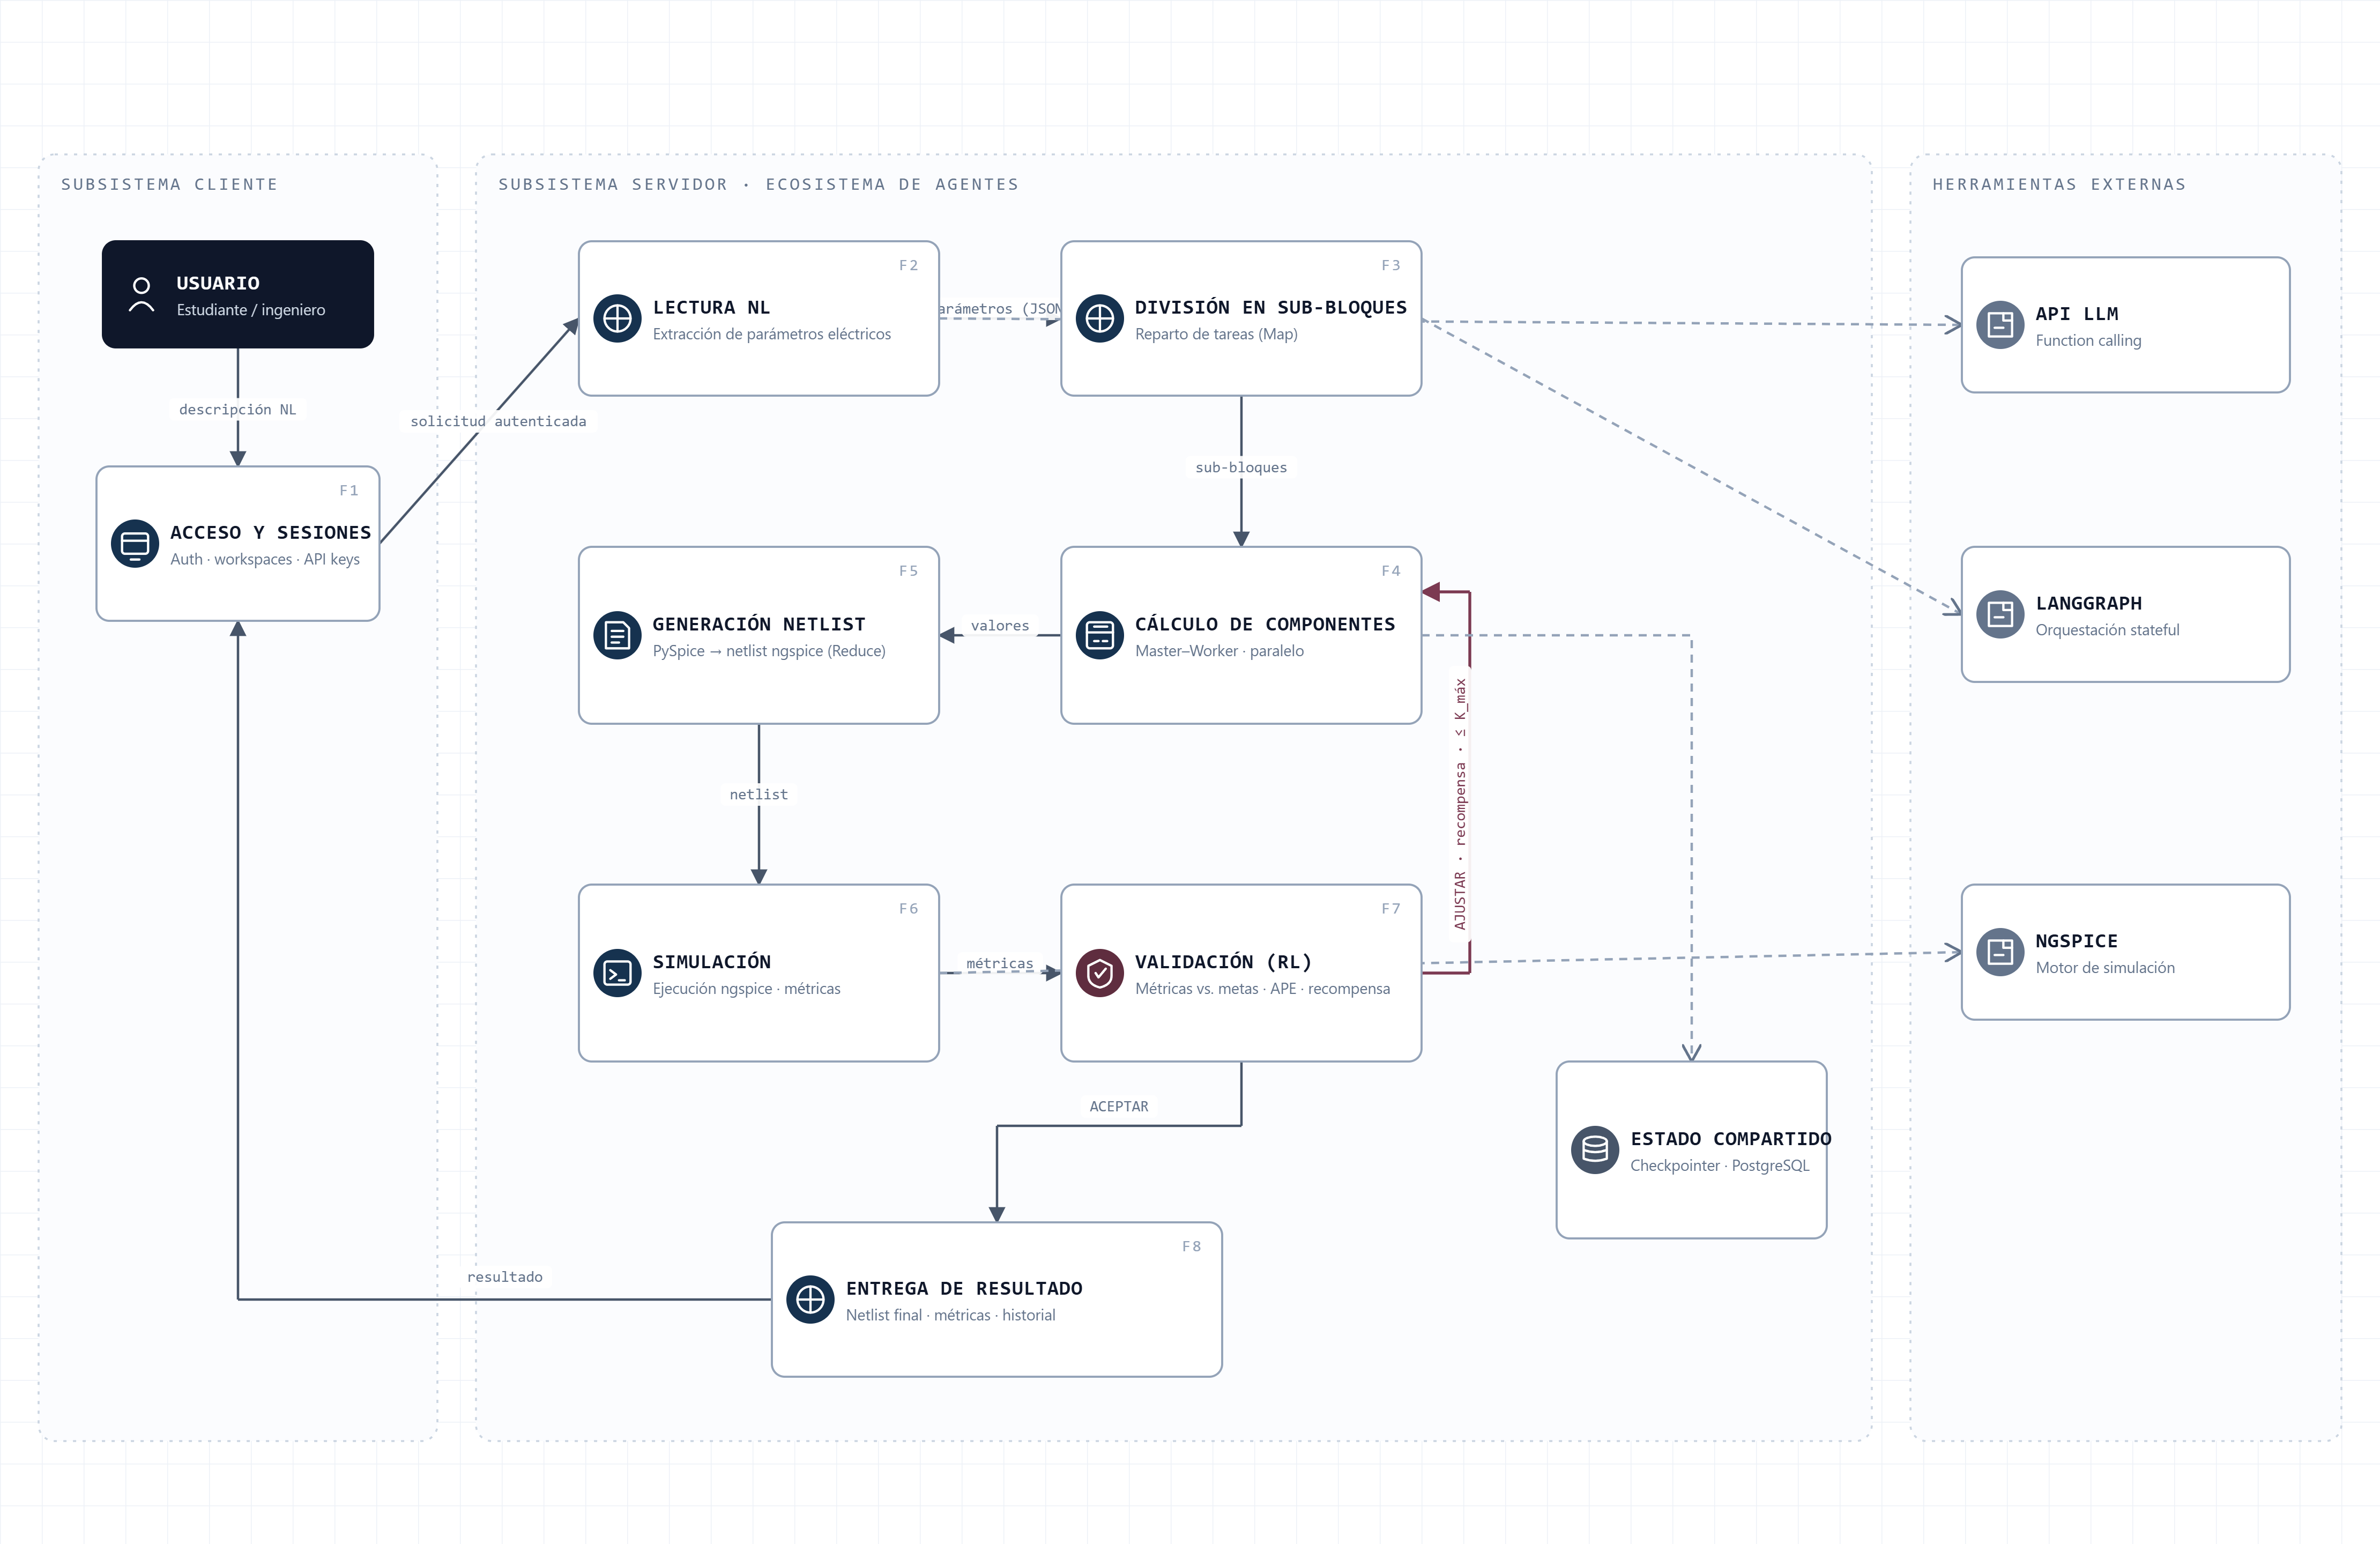
\includegraphics[width=1.3\textwidth, keepaspectratio]{../src/diagrams/diagrama_funcional.png}%
    }
    \caption{Diagrama funcional del sistema.}
    \label{fig:diagrama-funcional}
\end{figure}

\subsection{Modelo de casos de uso}
\label{subsec:prop-casos-uso}

Los casos de uso describen las interacciones que los actores ejecutan sobre el sistema. Se identifican dos clases de actor: el \textbf{usuario}, que interactúa con el subsistema cliente, y los \textbf{servicios externos} (la API del LLM y el motor ngspice), que el subsistema servidor consume durante la generación.

Los casos de uso principales del usuario incluyen: registrarse e iniciar sesión, gestionar espacios de trabajo, emitir y revocar API keys, y enviar una solicitud de generación de circuito junto con su descripción en lenguaje natural. El caso de uso central —\textit{generar circuito}— desencadena el flujo del subsistema servidor, que se detalla en su comportamiento dinámico en (sección~\ref{sec:prop-dinamico}). Los diagramas de casos de uso restantes (acceso, generación y decisión) se incluyen en el apéndice~\ref{apend:casos-uso}.

\begin{figure}[H]
    \centering
    \makebox[\textwidth][c]{%
        \hspace*{-0.5cm}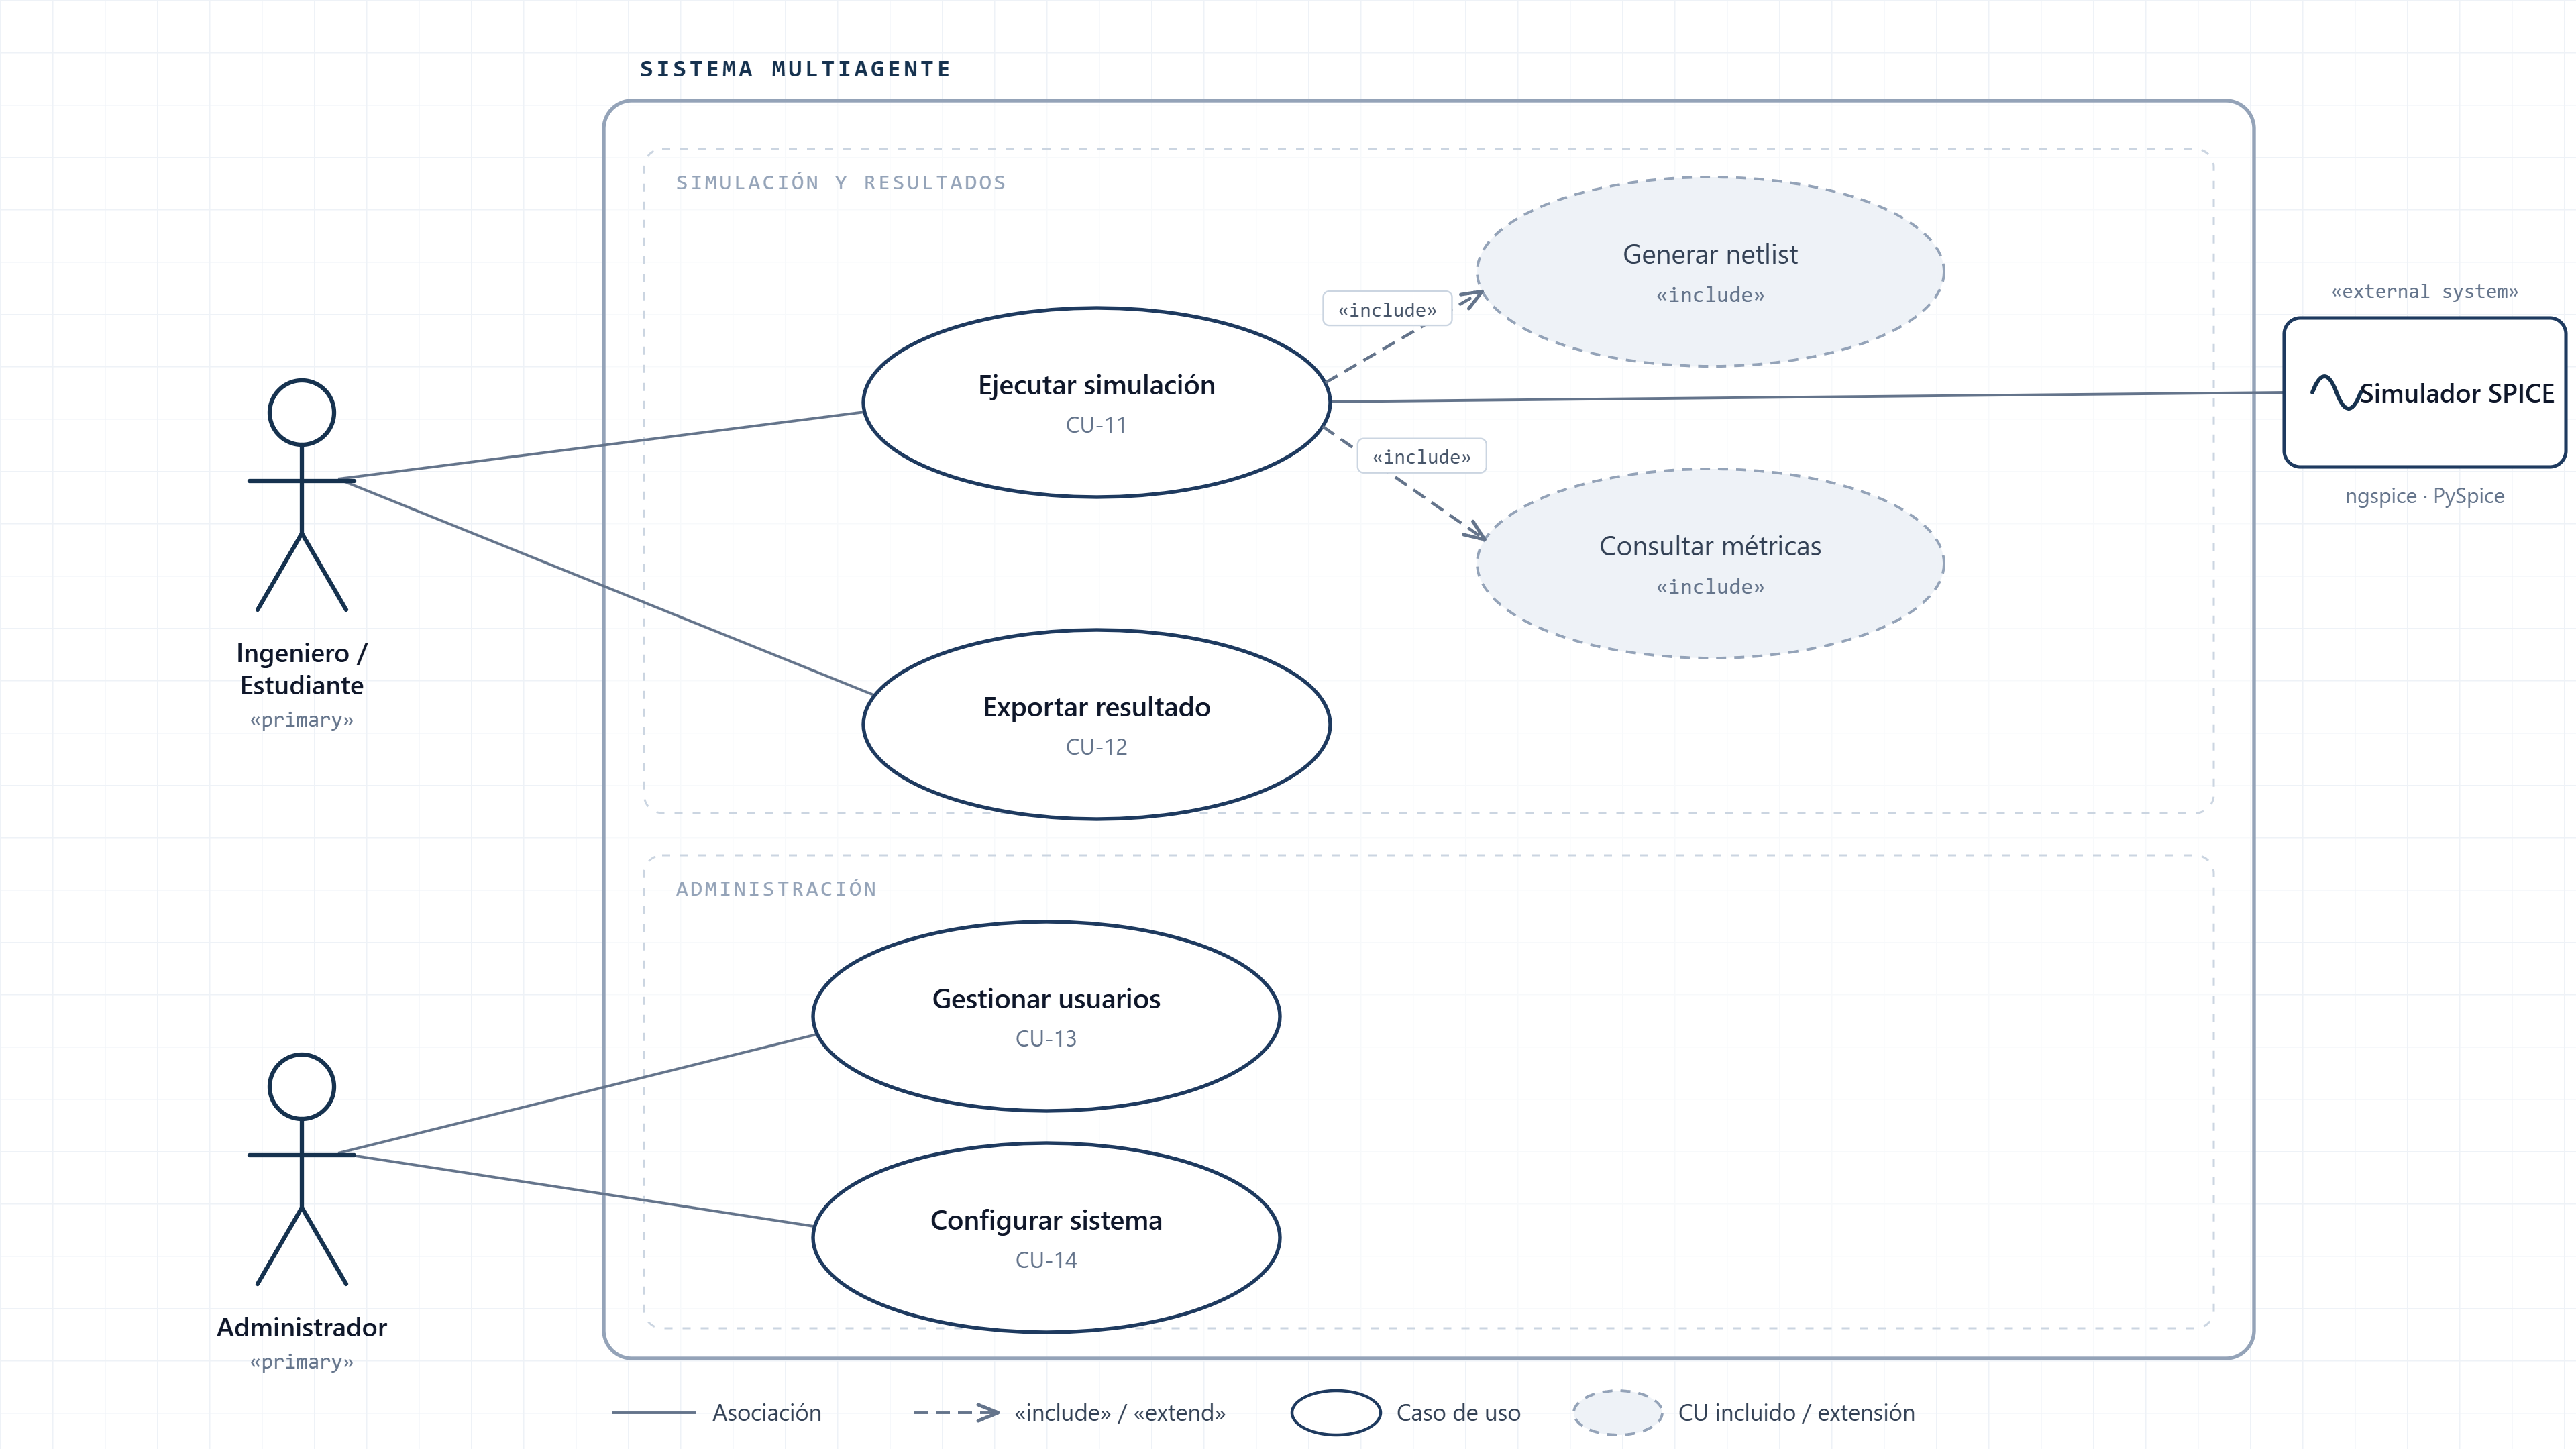
\includegraphics[width=1.3\textwidth, keepaspectratio]{../src/diagrams/casos_uso_simulacion.png}%
    }
    \caption{Diagrama de casos de uso: flujo de simulación y validación.}
    \label{fig:casos-uso-simulacion}
\end{figure}

\section{Arquitectura del sistema (modelo C4)}
\label{sec:prop-c4}

\subsection{Nivel 1 — Contexto}
\label{subsec:prop-c4-nivel1}

El nivel de contexto sitúa el sistema frente a sus actores y sistemas externos. Muestra al usuario interactuando con el sistema, y al sistema consumiendo dos servicios externos: la API del LLM y el motor de simulación ngspice. Este nivel deja claro que el sistema es una unidad que media entre la intención del usuario, expresada en lenguaje natural, y dos capacidades externas: el razonamiento del LLM y la simulación física del circuito.

\begin{figure}[H]
    \centering
    \makebox[\textwidth][c]{%
        \hspace*{-0.5cm}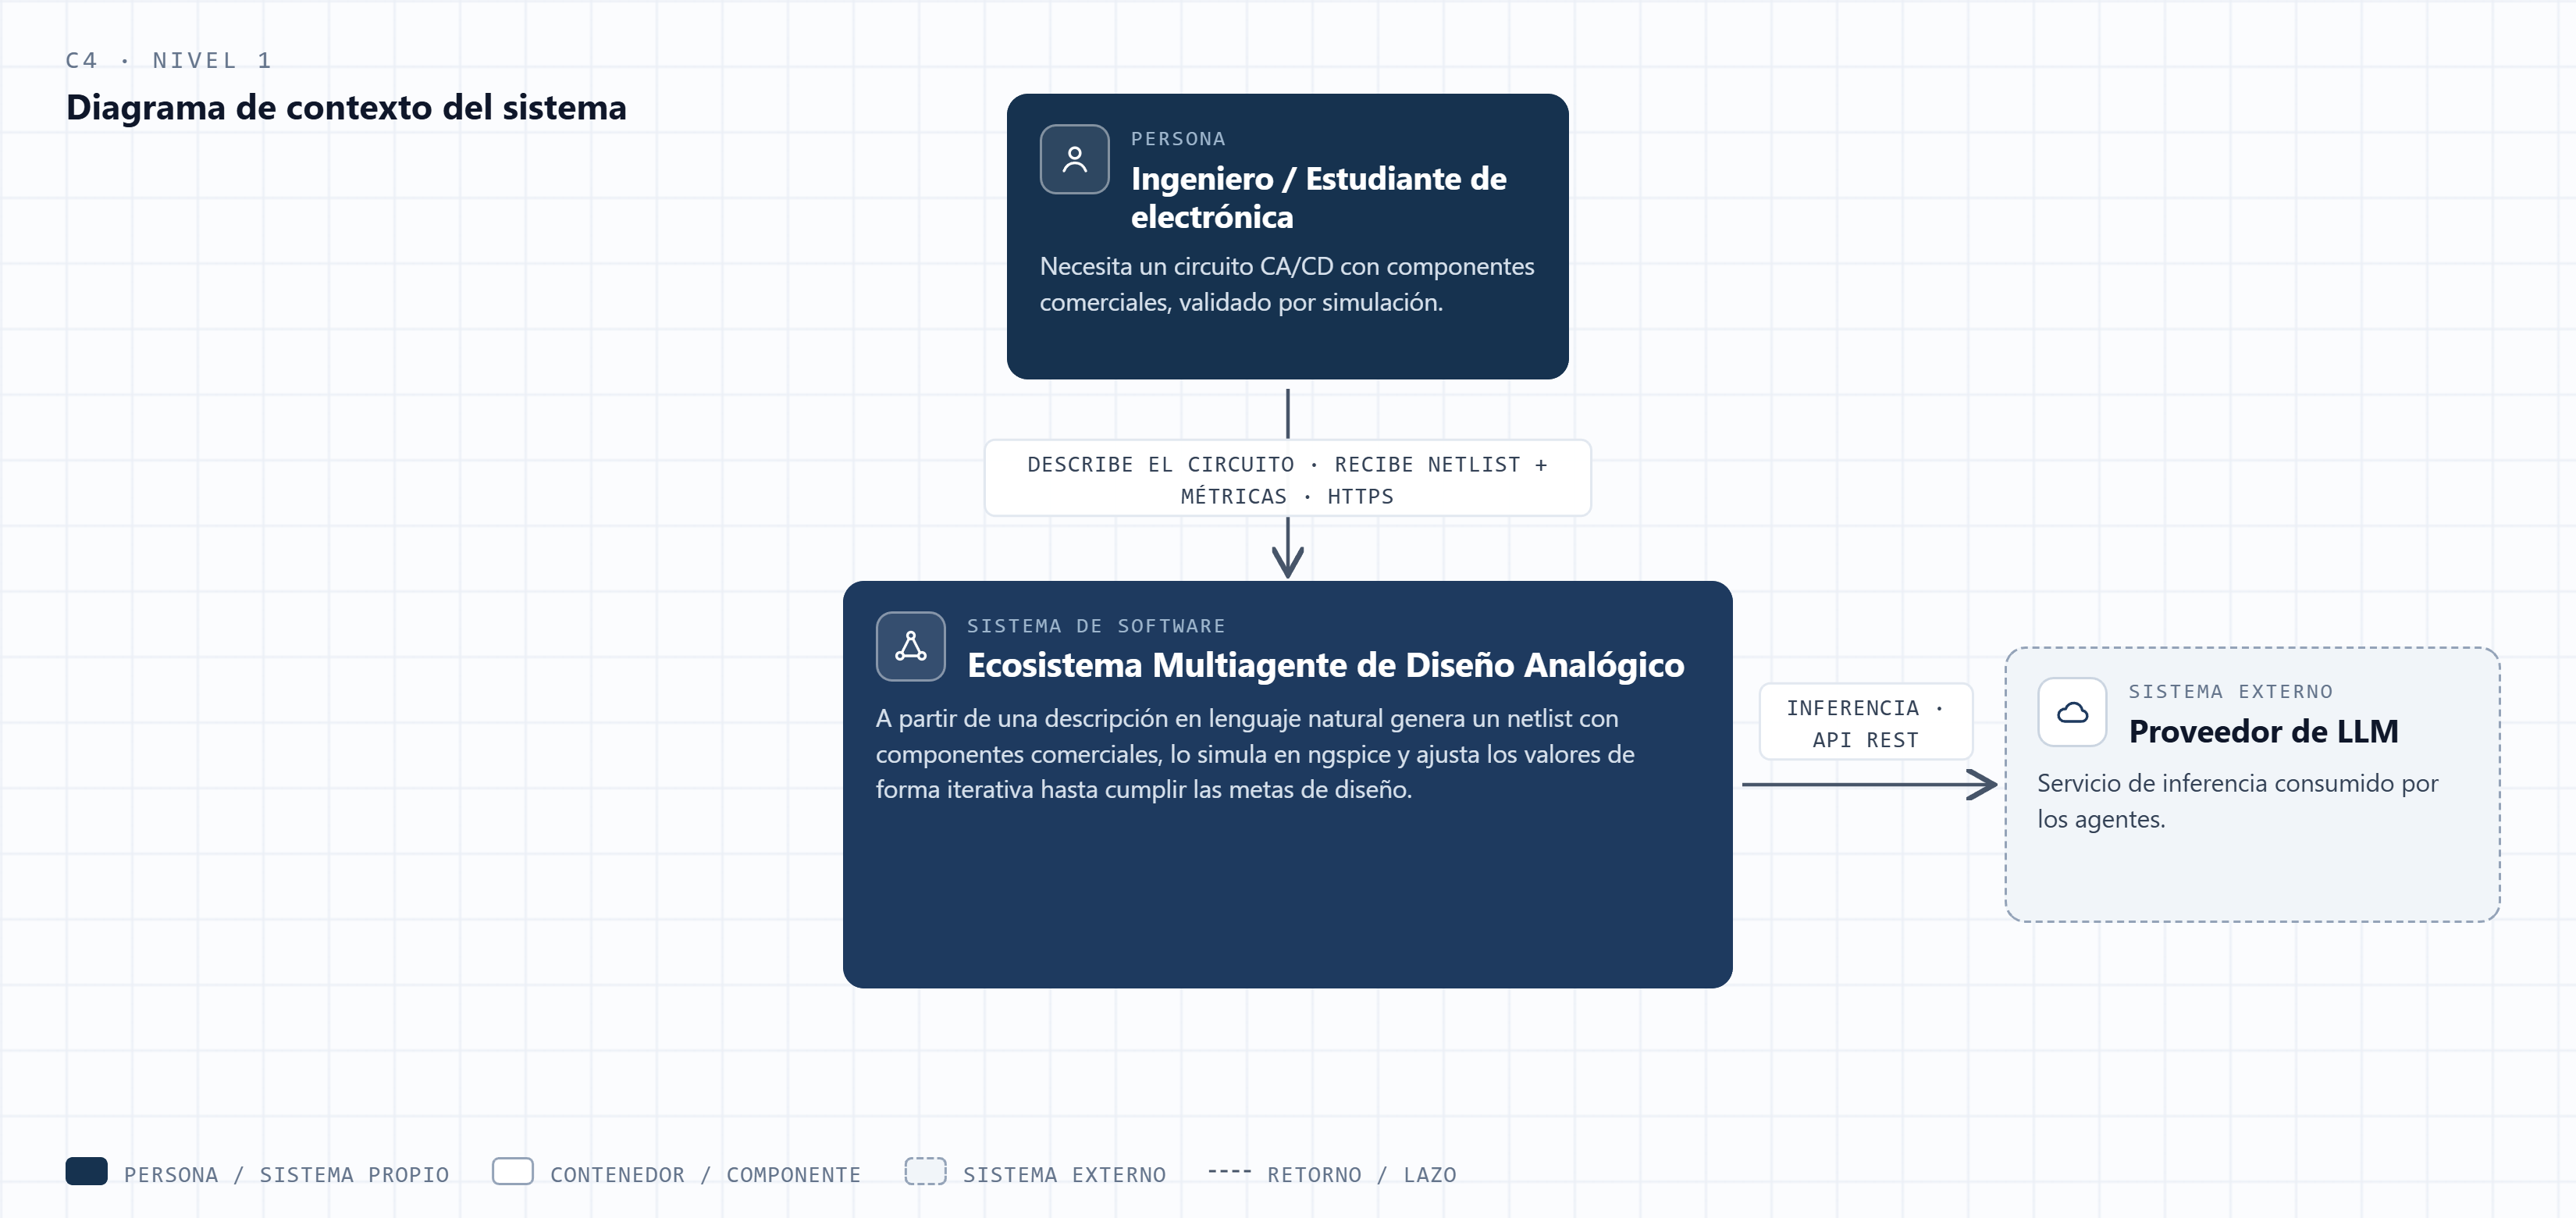
\includegraphics[width=1.3\textwidth, keepaspectratio]{../src/diagrams/c4_l1_v4.png}%
    }
    \caption{C4 Nivel 1: Diagrama de contexto.}
    \label{fig:c4-nivel1}
\end{figure}

\subsection{Nivel 2 — Contenedores}
\label{subsec:prop-c4-nivel2}

El nivel de contenedores descompone el sistema en sus unidades desplegables. Hace explícita la separación cliente/servidor: el subsistema cliente (autenticación, sesiones, espacios de trabajo, API keys) y el subsistema servidor (el ecosistema de agentes), junto con la base de datos de persistencia y la frontera con los servicios externos. Este nivel justifica la premisa de despliegue independiente (sección~\ref{subsec:prop-premisas-disenio}) y muestra el camino de una solicitud autenticada desde el cliente hacia el servidor.

\begin{figure}[H]
    \centering
    \makebox[\textwidth][c]{%
        \hspace*{-0.5cm}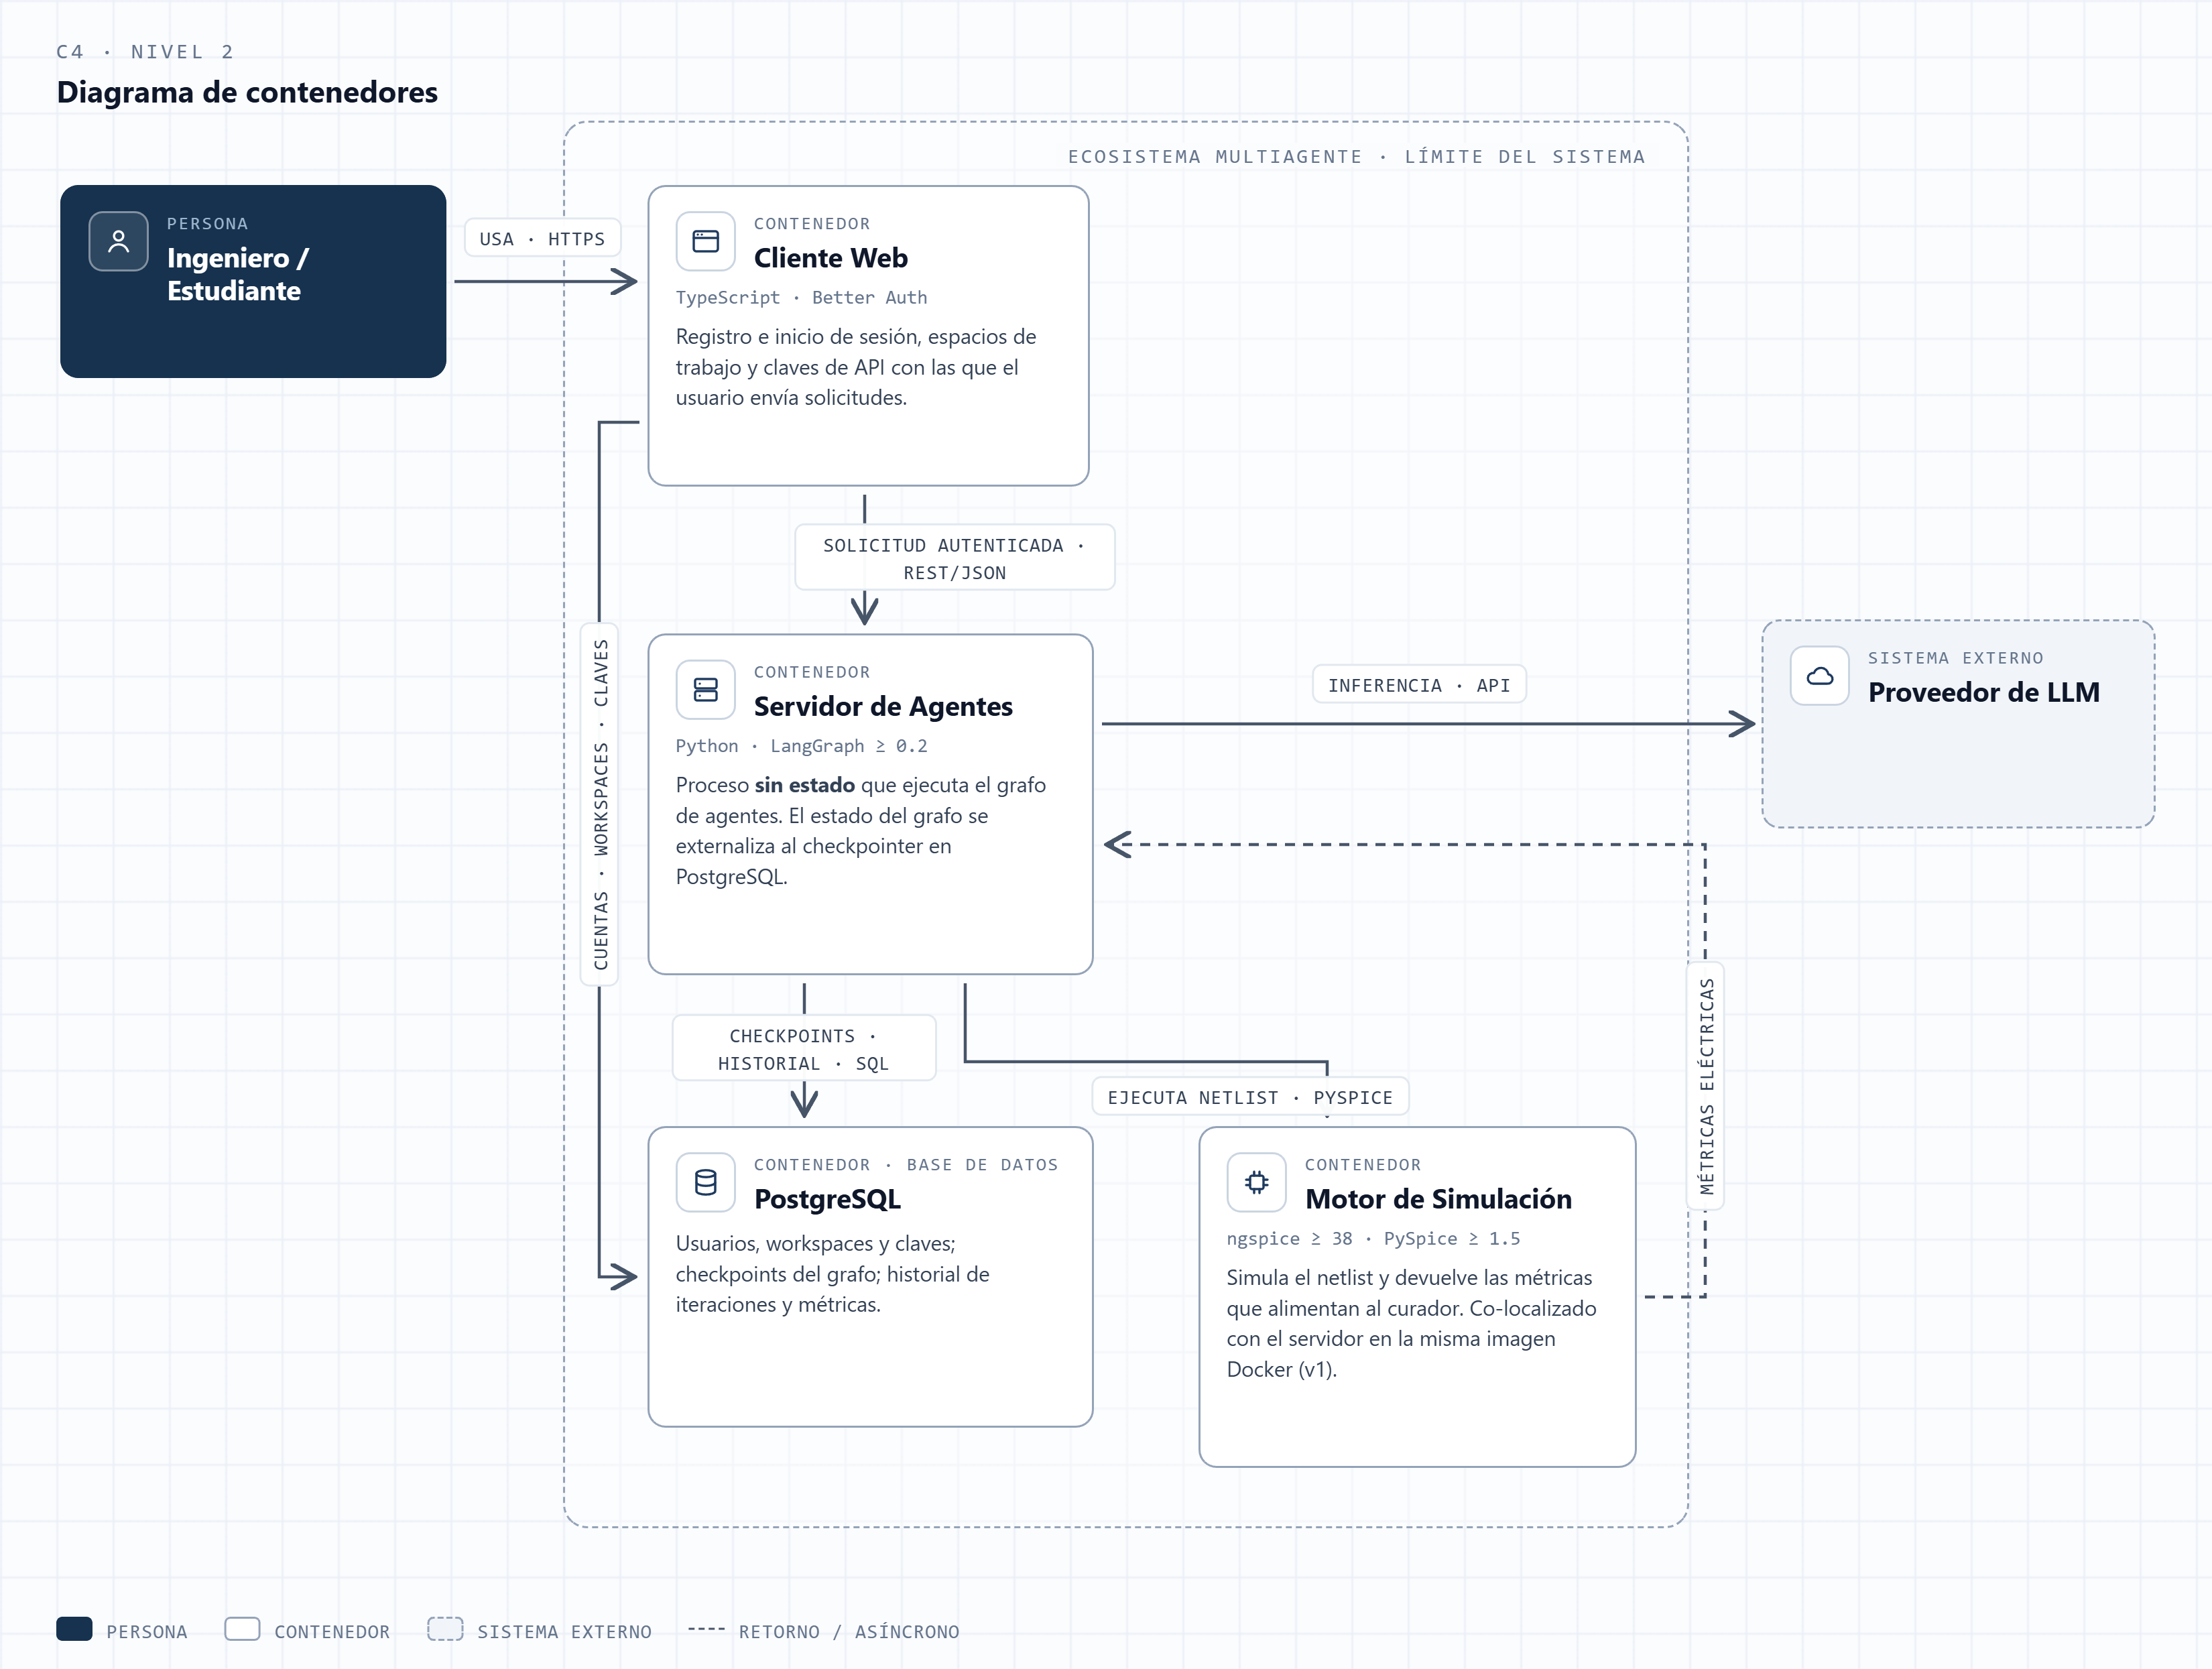
\includegraphics[width=1.3\textwidth, keepaspectratio]{../src/diagrams/c4_l2_v4.png}%
    }
    \caption{C4 Nivel 2: Diagrama de contenedores.}
    \label{fig:c4-nivel2}
\end{figure}

\subsection{Nivel 3 — Componentes}
\label{subsec:prop-c4-nivel3}

El nivel de componentes abre el subsistema servidor y muestra el ecosistema de agentes: el agente Orquestador (entrada del servidor y coordinador del estado compartido), el agente de Cálculo (Master-Worker), el agente Curador (RL, lazo de validación iterativa), el agente de Shell (ejecución de ngspice) y el agente de Escritura (generación del netlist con PySpice), todos coordinados sobre el grafo de orquestación con persistencia en base de datos. Este nivel materializa la premisa de modularidad de agentes (sección~\ref{subsec:prop-premisas-disenio}) y prepara el terreno para la descripción del comportamiento dinámico.

\begin{figure}[H]
    \centering
    \makebox[\textwidth][c]{%
        \hspace*{-0.5cm}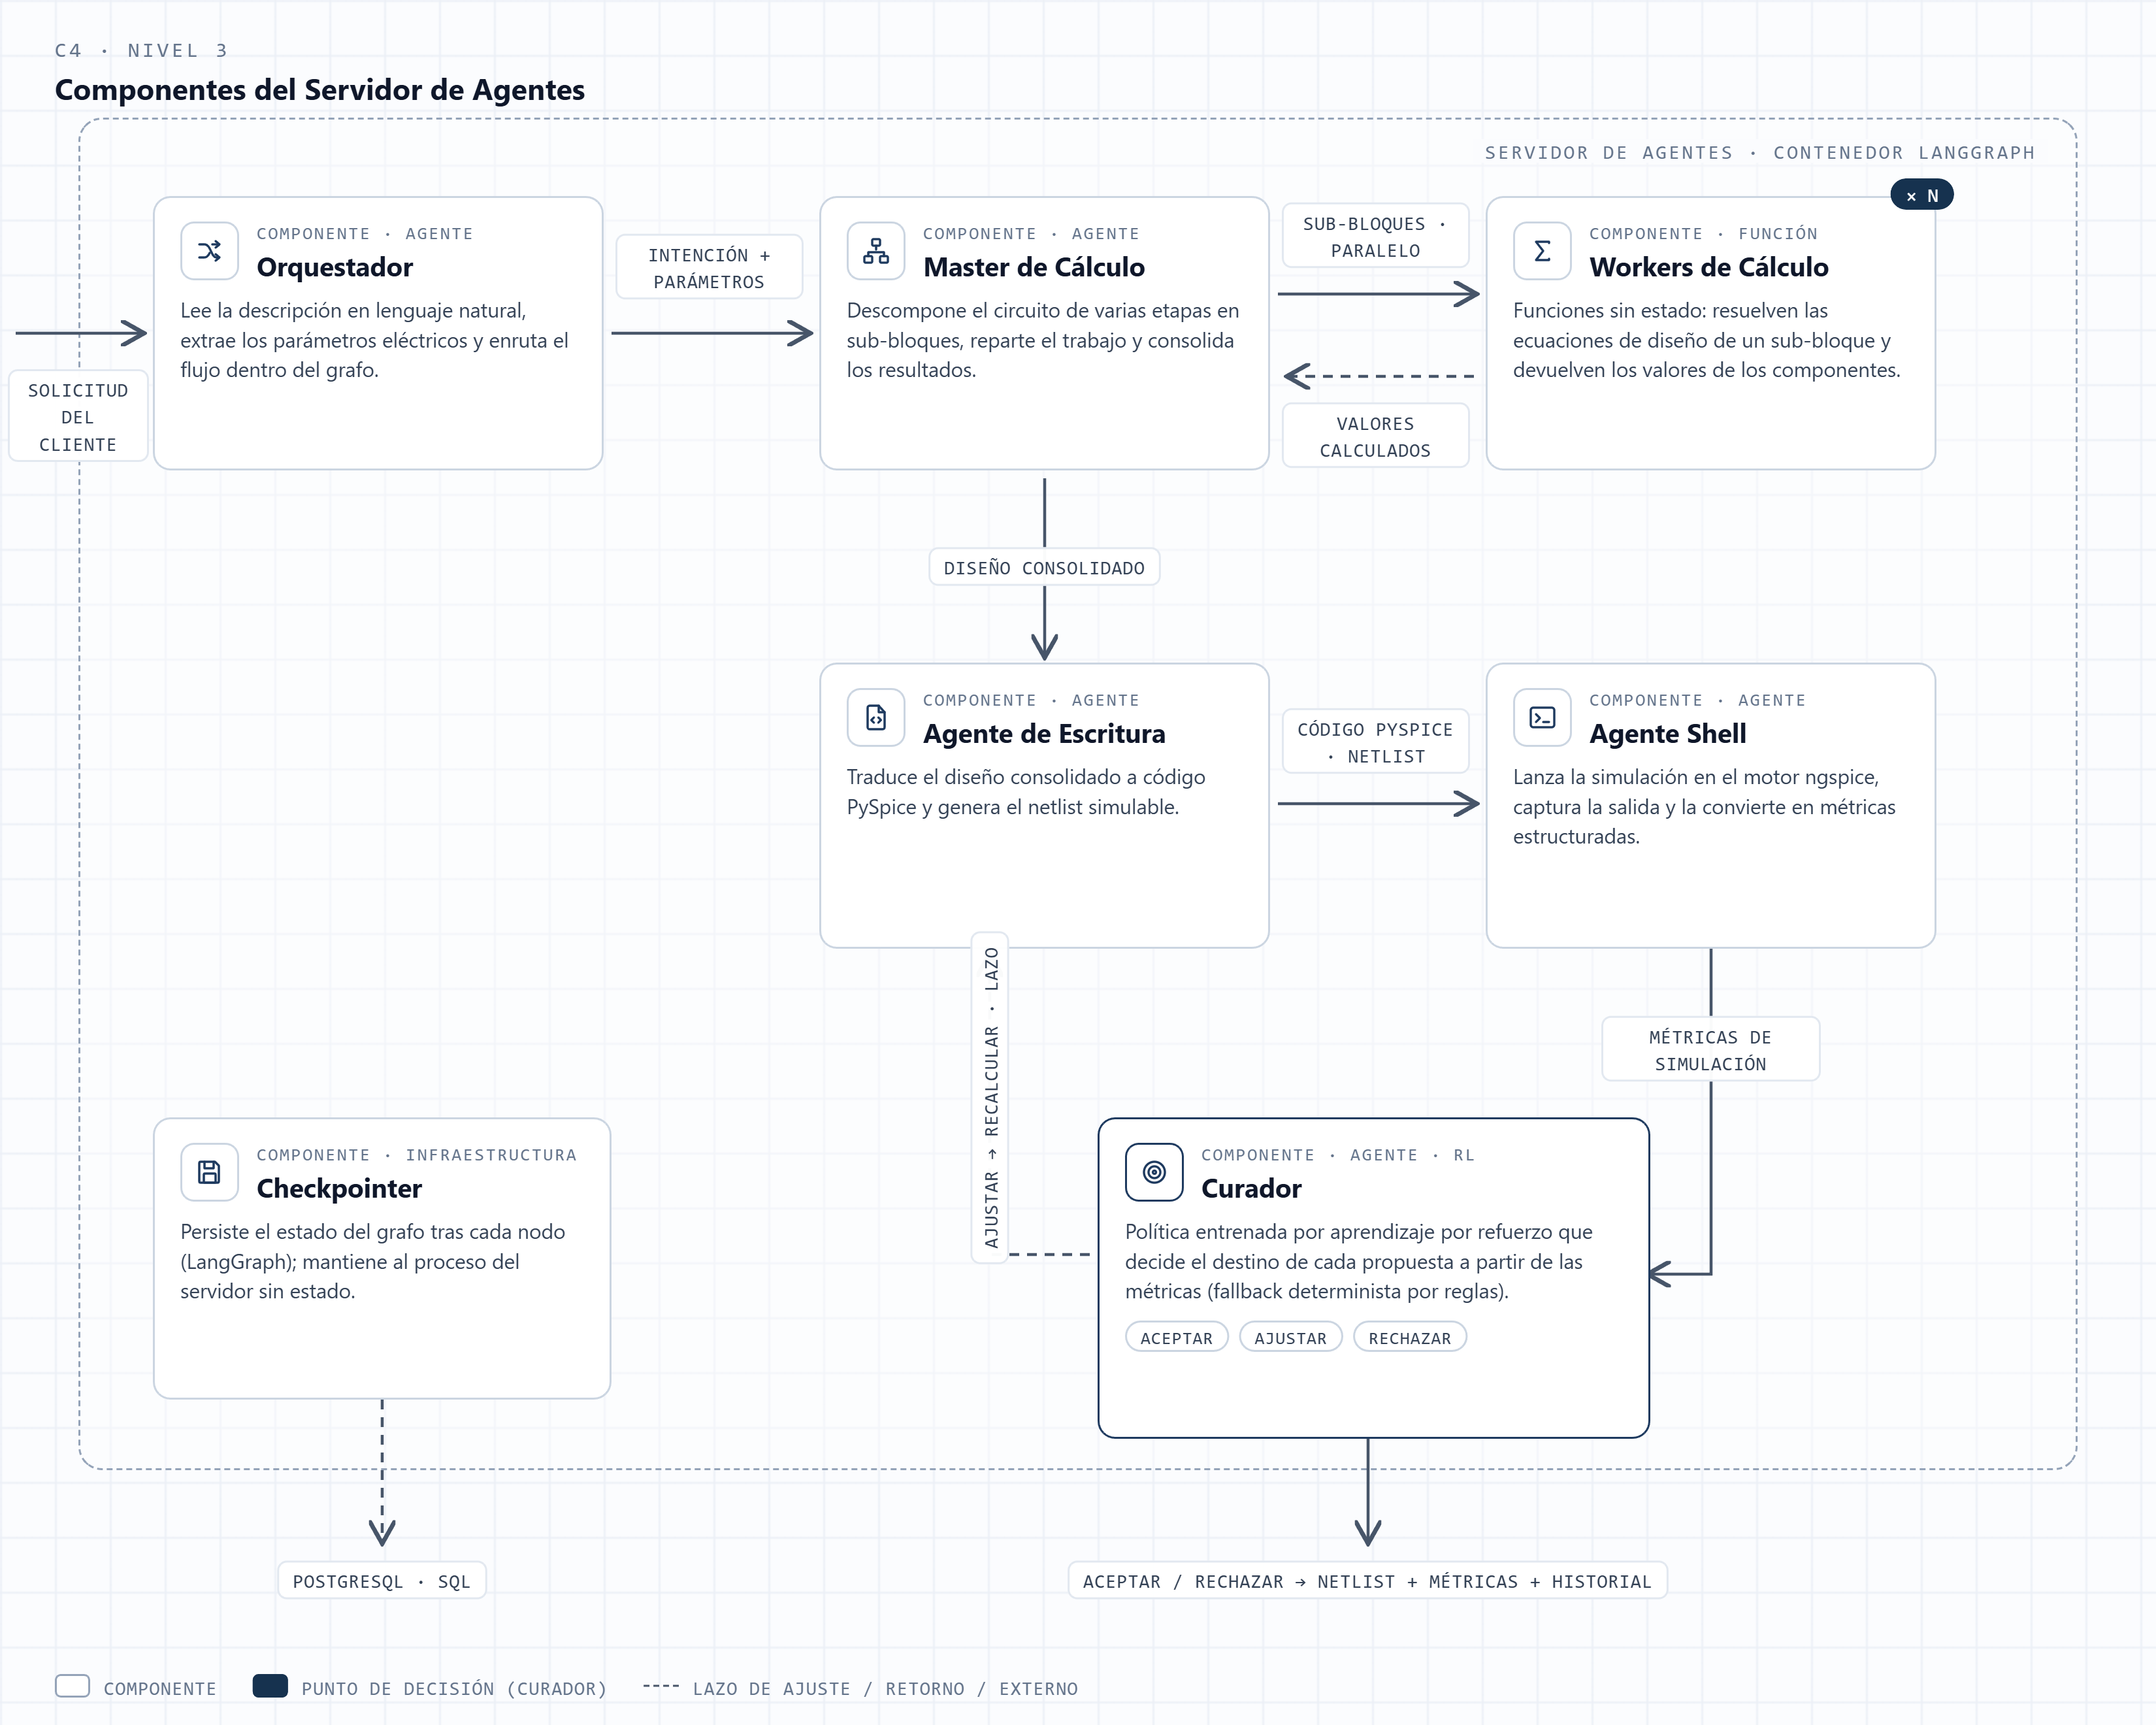
\includegraphics[width=1.3\textwidth, keepaspectratio]{../src/diagrams/c4_l3_v4.png}%
    }
    \caption{C4 Nivel 3: Diagrama de componentes.}
    \label{fig:c4-nivel3}
\end{figure}

\section{Comportamiento dinámico: flujo de generación}
\label{sec:prop-dinamico}

Las secciones anteriores describen la estructura estática del sistema. Esta sección describe su comportamiento en ejecución: cómo colaboran los agentes en el tiempo para transformar una descripción en lenguaje natural en un netlist validado. El diagrama de secuencia integra las vistas anteriores en una línea temporal.

El flujo principal procede así: el orquestador recibe la solicitud autenticada y la descripción del circuito, usa el LLM para extraer los parámetros y la lista de sub-bloques, y reparte los sub-bloques independientes en paralelo al agente de cálculo (Master-Worker). El agente de escritura genera el código PySpice y el netlist; el agente de shell lo simula en ngspice y lee las métricas; el agente curador compara las métricas con las metas y decide. Según su decisión, el ciclo se repite —ajustando los valores— o termina. El ciclo está acotado por un número máximo de iteraciones configurable (parámetro de guarda del lazo).

El comportamiento de persistencia se modela de forma explícita: el estado de cada iteración se conserva mediante el \textit{checkpointer}, lo que se representa como un fragmento de referencia en el diagrama, de modo que la naturaleza con estado del sistema quede formalmente reflejada y no como una observación accesoria.

\begin{figure}[H]
    \centering
    \makebox[\textwidth][c]{%
        \hspace*{-0.5cm}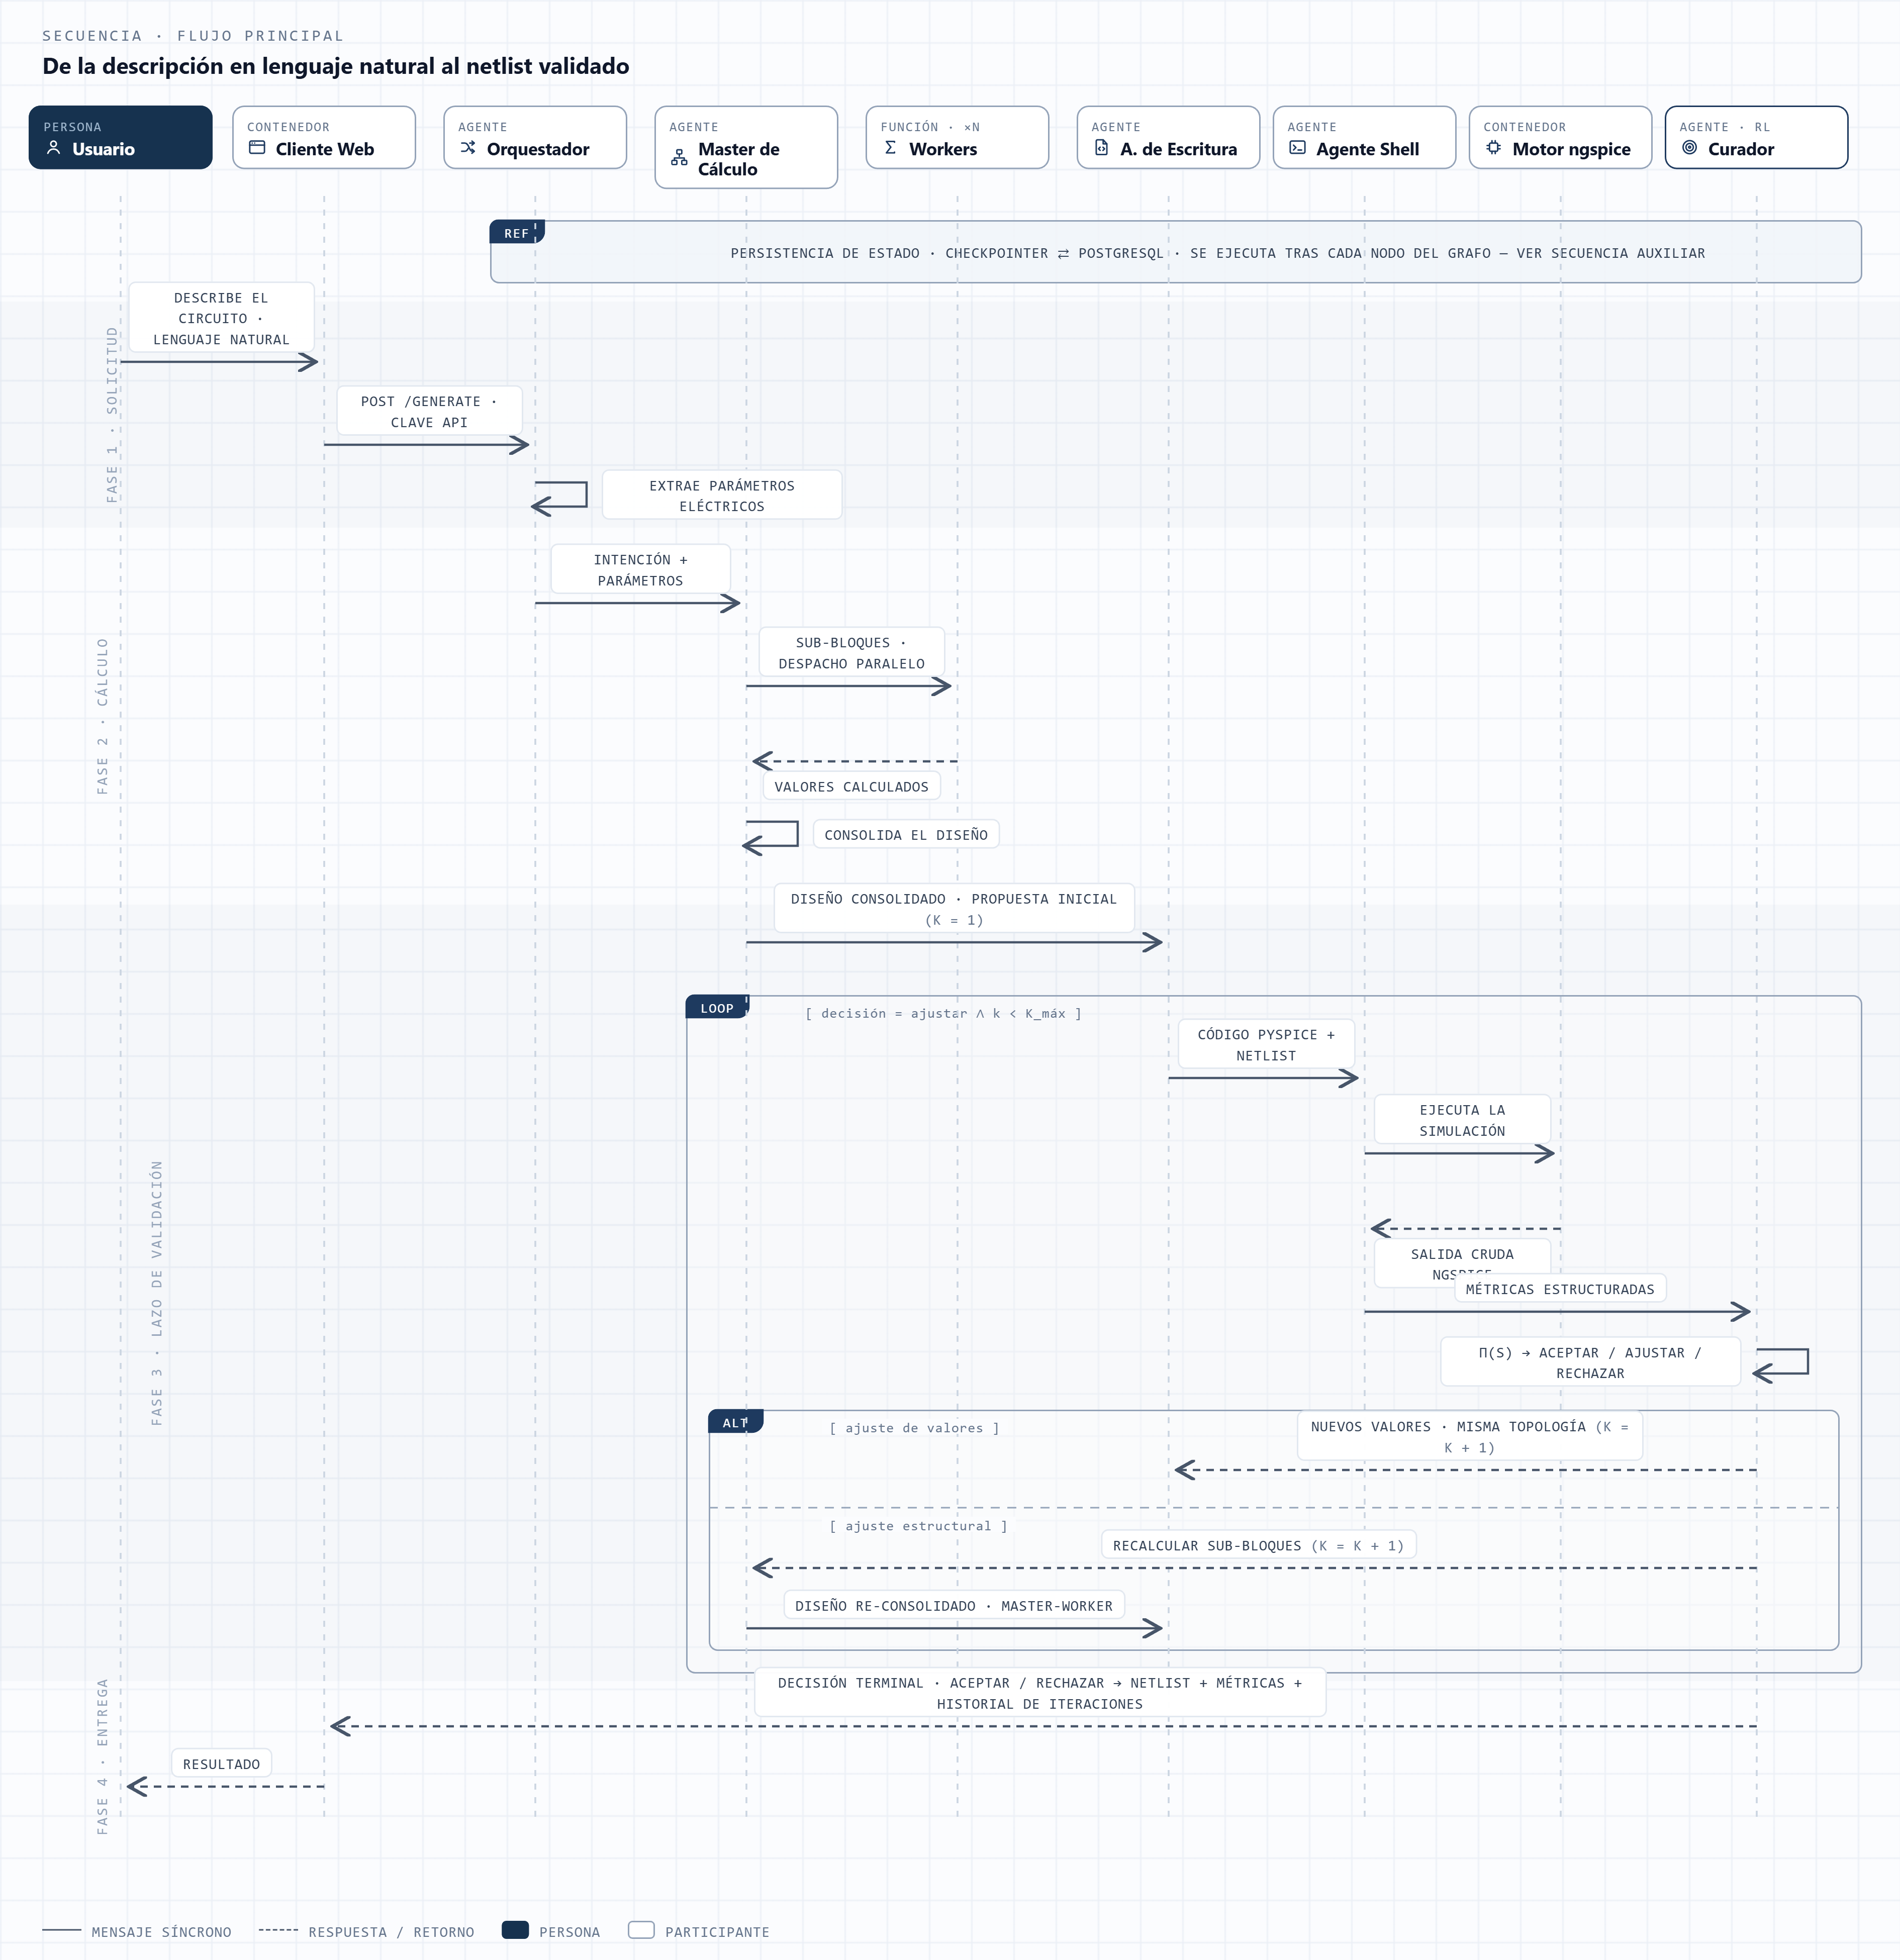
\includegraphics[width=1.3\textwidth, keepaspectratio]{../src/diagrams/secuencia_flujo_principal.png}%
    }
    \caption{Diagrama de secuencia del flujo de generación.}
    \label{fig:secuencia-generacion}
\end{figure}

\section{Calidad de la solución}
\label{sec:prop-calidad}

La calidad de la solución se entiende aquí como el grado en que el sistema satisface las necesidades para las que se diseña, evaluado sobre características observables y no sobre el juicio del diseñador. El modelo de calidad del producto de la norma ISO/IEC 25010 organiza esas características y ofrece un vocabulario común para nombrarlas \cite{iso_25010}. Se adopta el modelo de calidad del producto ---y no el de calidad en uso, centrado en la experiencia del usuario final--- porque el sistema se evalúa como un artefacto técnico operado mediante una interfaz de programación. De las características que define la norma, el diseño atiende de forma directa cinco: idoneidad funcional, fiabilidad, eficiencia de desempeño, mantenibilidad y seguridad. A ellas se suma la trazabilidad de la generación, que el SRS recoge como requisito no funcional. Cada atributo se apoya en una decisión de diseño ya expuesta y su comprobación se registra como criterio de aceptación o como requisito no funcional, cuya medición corresponde al capítulo de pruebas.

La idoneidad funcional expresa si el sistema hace lo que debe: generar, a partir de una descripción en lenguaje natural, un circuito analógico CA/CD cuyos parámetros se acercan a las metas. Esta característica es la razón de ser del sistema y se concreta en métricas que la hacen medible ---la tasa de resolución y el error porcentual absoluto medio---, contrastadas además frente a una línea base \textit{best-of-N}. El lazo de ajuste guiado por el curador es el mecanismo que la persigue: itera hasta acercar las métricas a las metas o hasta agotar el número de iteraciones.

La fiabilidad se refiere a que el sistema se comporte de forma estable ante las condiciones esperadas y ante el fallo. El diseño la atiende por tres vías. El lazo de ajuste está acotado por un número máximo de iteraciones, lo que impide que el proceso se prolongue de forma indefinida ante un circuito que no converge. El curador dispone de una decisión determinista por reglas como respaldo de su política, de modo que el sistema produce siempre una decisión aunque la política aprendida no resulte aplicable. Y el \textit{checkpointer} aporta recuperabilidad: al persistir el estado de la generación tras cada paso, una ejecución interrumpida puede retomarse desde el último punto guardado en lugar de reiniciarse, propiedad que el SRS recoge como tolerancia a fallos (RNF-03.2). La convergencia de la simulación se registra como una métrica y forma parte del estado que el curador evalúa, lo que evita que un netlist no convergente se acepte como válido.

La eficiencia de desempeño atañe al tiempo y a los recursos que el sistema consume para producir un resultado. El diseño la aborda mediante el cálculo concurrente de los sub-bloques independientes, que reduce la latencia frente a un cálculo secuencial, y mediante un límite de tiempo para el ciclo completo. El carácter sin estado del subsistema servidor habilita además su réplica detrás de un balanceador de cargas, lo que permite atender más solicitudes en paralelo sin rediseñar el sistema; esta capacidad de crecer mediante réplicas es lo que el SRS registra como escalabilidad y que el modelo de la norma sitúa dentro de la eficiencia de desempeño.

La mantenibilidad se fundamentó ya entre las premisas de diseño (sección~\ref{subsec:prop-premisas-disenio}): la modularidad de los agentes materializa la alta cohesión y el bajo acoplamiento, y la configuración externa de los pesos, los factores y los umbrales del curador permite ajustar el comportamiento del sistema sin tocar el código. Se retoma aquí para situarla dentro del modelo de calidad, no para repetir su justificación.

A la mantenibilidad se vincula la trazabilidad de la generación. El sistema conserva el historial de iteraciones y la recompensa que el curador calcula en cada ciclo, de modo que el camino que llevó a un netlist queda registrado y es posible reconstruirlo. En términos del modelo de la norma, esta propiedad se aproxima a la analizabilidad, una faceta de la mantenibilidad, pues facilita diagnosticar el comportamiento del sistema tras una ejecución. El mismo registro constituye la traza en la que se apoya el control de seguridad descrito en la sección~\ref{sec:prop-seguridad}, lo que enlaza la calidad y la seguridad sobre un único mecanismo.

La seguridad es, en el modelo ISO/IEC 25010, una característica de calidad más. Por su peso en un sistema que gestiona credenciales y claves de acceso, se trata de forma separada en la sección siguiente.

La correspondencia entre cada característica, la decisión de diseño que la atiende y el lugar donde se registra o se mide se resume a continuación.

\begin{table}[H]
\centering
\small
\caption{Correspondencia entre atributos de calidad, decisiones de diseño y evidencia de evaluación.}
\label{tab:calidad-solucion}
\vspace{0.3cm}
\renewcommand{\arraystretch}{1.35}
\rowcolors{2}{white}{rowgray}
\begin{tabularx}{\textwidth}{p{3.1cm} >{\raggedright\arraybackslash}X >{\raggedright\arraybackslash}X}
\toprule
\rowcolor{guinda}
\textcolor{white}{\textbf{Característica}} &
\textcolor{white}{\textbf{Decisión de diseño que la atiende}} &
\textcolor{white}{\textbf{Dónde se registra o mide}} \\
\midrule
Idoneidad funcional & Lazo de ajuste guiado por el curador & Tasa de resolución y MAPE; comparación con \textit{best-of-N} \\
Fiabilidad & Límite de iteraciones; respaldo determinista del curador; recuperabilidad por \textit{checkpointer}; registro de convergencia & CA-04, CA-05; RNF-03.2 \\
Eficiencia de desempeño & Cálculo concurrente; límite de tiempo; servidor sin estado replicable & RNF-01.1, RNF-01.2; CA-05, CA-06 \\
Mantenibilidad & Modularidad de los agentes; configuración externa & RNF-04.1 \\
Trazabilidad (analizabilidad) & Registro del historial de iteraciones y de la recompensa & CA-03; RNF de trazabilidad \\
Seguridad & Controles descritos en la sección~\ref{sec:prop-seguridad} & RF-06, RIMP-11 \\
\bottomrule
\end{tabularx}
\end{table}

Conviene precisar el alcance de esta evaluación de calidad. La idoneidad funcional, la fiabilidad y la eficiencia de desempeño se contrastan contra umbrales numéricos en el capítulo de pruebas. La mantenibilidad, la trazabilidad y la seguridad, en cambio, se evidencian de forma estructural ---por las propiedades del diseño y por la revisión del código y del repositorio--- y no mediante una métrica cuantitativa, lo que constituye un límite reconocido de la evaluación. Quedan fuera del foco de calidad de esta versión la usabilidad ---el sistema se opera mediante una interfaz de programación, no mediante una interfaz gráfica para usuarios finales--- y la portabilidad más allá del despliegue reproducible en contenedores.

\section{Seguridad de la solución}
\label{sec:prop-seguridad}

La seguridad del sistema se aborda en proporción a su naturaleza de prototipo académico: el objetivo no es una auditoría completa, sino controles razonables sobre los activos que el sistema maneja. Esos activos son las credenciales de los usuarios, las API keys con las que se autentican las solicitudes, los secretos del propio sistema ---la clave de la API del LLM, las credenciales de la base de datos y los secretos de Better Auth---, las descripciones y netlists de cada usuario y la integridad del estado que el servidor persiste durante la generación. El análisis se ordena con los tres principios clásicos de la seguridad informática: confidencialidad, integridad y disponibilidad \cite{stallings2018computer}.

Bajo confidencialidad se agrupan los secretos y las credenciales, que no deben quedar expuestos. A esta categoría pertenece también la descripción del circuito que el usuario envía, que el sistema transmite a un proveedor de LLM externo para su procesamiento; la confidencialidad de esos datos depende en parte de ese proveedor, dependencia que se reconoce como límite al final de la sección. La integridad se refiere a que el estado de una generación y el netlist resultante no se alteren de forma indebida entre iteraciones. La disponibilidad ---que el servicio responda a las solicitudes legítimas--- se apoya en el diseño sin estado del servidor, que admite réplicas y reduce el impacto de la caída de una instancia.

El diseño incorpora un conjunto de controles proporcionados a esos activos. La autenticación de los usuarios se delega en Better Auth \cite{betterauth}, que concentra el registro, el inicio de sesión y la gestión de sesiones en un componente especializado en lugar de implementarlos desde cero. La autorización de las solicitudes al servidor se realiza mediante API keys que el usuario emite y puede revocar, de modo que cada solicitud que llega al servidor viaja autenticada. Las API keys y los circuitos de cada usuario quedan acotados a su espacio de trabajo, por lo que la autorización no se limita a comprobar que una solicitud esté autenticada, sino a que cada usuario acceda solo a sus propios recursos. La separación entre subsistema cliente y subsistema servidor actúa como frontera de confianza: el servidor no expone la lógica de diseño a solicitudes no autenticadas y el cliente no ejecuta esa lógica. Los secretos del sistema se leen de variables de entorno y no se escriben en el código ni se versionan en el repositorio, control que el SRS recoge como requisito de manejo de secretos (RIMP-11).

Un riesgo propio de un sistema que recibe lenguaje natural y lo entrega a agentes basados en LLM es que la entrada del usuario contenga instrucciones que desvíen el comportamiento de los agentes. Para acotarlo, la descripción se valida y se restringe a los parámetros eléctricos que el orquestador necesita antes de incorporarla al proceso, y la salida del modelo se exige en un formato estructurado, lo que reduce el margen para respuestas fuera de lo previsto.

Un control específico de este sistema atiende la ejecución de artefactos producidos por el modelo. El agente de escritura genera código PySpice y un netlist, y el agente de shell los ejecuta para obtener las métricas; ejecutar código generado por un LLM es una superficie que conviene contener. El diseño la acota al ejecutar esos artefactos dentro del entorno contenedorizado del servidor, cuyo despliegue reproducible recoge el SRS (RIMP-10), de modo que la ejecución queda aislada del entorno anfitrión. El endurecimiento de ese aislamiento más allá de la contención por contenedor queda fuera del alcance de esta versión. El registro de la actividad ---entre otros, la recompensa que el curador calcula en cada iteración--- deja una traza que permite revisar el comportamiento del sistema tras una ejecución.

Los controles anteriores se corresponden con varias de las categorías de riesgo que recopila el proyecto OWASP en su lista de los diez riesgos más críticos para aplicaciones web \cite{owasp_top10}. El control de acceso por API key y el aislamiento entre espacios de trabajo atienden el riesgo de control de acceso roto; la delegación en Better Auth, el de fallos de identificación y autenticación; el manejo de secretos fuera del repositorio, el de configuración de seguridad deficiente y exposición de datos sensibles; la validación de la entrada, el de inyección; y la contención de la ejecución de artefactos generados, el de fallos de integridad del software y de los datos. La lista de OWASP se emplea como catálogo de referencia para situar los controles, no como una verificación exhaustiva de conformidad.

El alcance de seguridad de esta versión tiene límites explícitos. La comunicación entre el usuario y el sistema se realiza sobre HTTPS, pero el diseño no incorpora cifrado de los datos en reposo más allá del que provea la base de datos, ni monitoreo de seguridad especializado, ni pruebas de penetración formales, ni un modelado de amenazas exhaustivo. A ello se añaden dos límites particulares: el sistema no aplica un control de tasa sobre las solicitudes, por lo que el uso intensivo de un usuario autenticado puede consumir recursos de cómputo y llamadas al LLM sin freno; y la confidencialidad de los datos enviados al proveedor de LLM externo escapa al control directo del sistema. Todos ellos exceden el alcance de un prototipo de tesina y se señalan para delimitar con honestidad qué protege el sistema y qué no.

\section{Criterios de aceptación de la propuesta}
\label{sec:prop-criterios}

La propuesta de solución se considerará satisfactoria si el sistema construido cumple un conjunto de criterios de aceptación objetivos y comprobables de forma independiente. Estos criterios están enunciados en el SRS junto con su procedimiento de verificación, lo que permite contrastarlos con mediciones reales en lugar de con el juicio del diseñador. No se evalúan en este capítulo —su comprobación empírica corresponde al capítulo de experimentos y resultados— pero se enuncian aquí como cierre del diseño, para dejar explícito qué deberá medirse y bajo qué condición se dará por cumplido.

Entre los criterios relevantes figuran: que el sistema acepte una descripción en lenguaje natural y extraiga de ella correctamente los parámetros eléctricos; que ejecute sub-bloques independientes en paralelo; que el lazo de ajuste itere hasta cumplir la meta o alcanzar el máximo de iteraciones; que produzca un netlist simulado en ngspice; y que la salida sea repetible con la temperatura del LLM fijada, para permitir la comparación de resultados durante la evaluación.

\section{Síntesis del diseño}
\label{sec:prop-sintesis}

La propuesta de solución descrita en este capítulo da forma concreta a la brecha identificada en el estado del arte: un sistema que genera y valida circuitos analógicos CA/CD a nivel de componentes comerciales, con la simulación SPICE incorporada dentro del lazo de diseño. El diseño se articula en tres planos que se sostienen entre sí. La descomposición funcional y los casos de uso (sección~\ref{sec:prop-funcional}) establecen qué hace el sistema y quién interactúa con él. El modelo C4 en sus tres niveles (sección~\ref{sec:prop-c4}) establece cómo se estructura: la separación en subsistema cliente y subsistema servidor, y la organización del servidor como un ecosistema de agentes modulares —Orquestador, Cálculo, Curador, Shell y Escritura— coordinados sobre un grafo con estado y persistencia. El diagrama de secuencia (sección~\ref{sec:prop-dinamico}) establece cómo se comportan esos elementos en el tiempo, integrando el lazo de ajuste iterativo que distingue a la propuesta.

Los criterios de aceptación enunciados en (sección~\ref{sec:prop-criterios}) fijan la condición que el sistema construido deberá cumplir. Su comprobación —la medición del comportamiento del sistema frente a esos criterios sobre un conjunto de circuitos de prueba— constituye la evaluación del sistema y se desarrolla en el capítulo siguiente, que toma este diseño como objeto de medida.
